\documentclass{beamer}

\mode<presentation>
{
 \usetheme{Boadilla}
 \setbeamercovered{transparent}}

\usepackage[english]{babel}
\usepackage{times}

\usepackage{xcolor}
\usepackage{colortbl}
%\usepackage{subfigure}

\usepackage{fontspec} 
\usepackage{xunicode}
\usepackage{xltxtra}
\usepackage{booktabs}
\newenvironment{CJK}{\fontspec[Scale=0.9]{PMingLiU}}{}
\newenvironment{Geeza}{\fontspec[Scale=0.9]{Geeza Pro}}{}

%% for tables
\newcommand{\mc}{\multicolumn}
\newcommand{\lab}[1]{\multicolumn{1}{c}{#1}}
\newcommand{\ind}[1]{{\fboxsep1pt\raisebox{-.5ex}{\fbox{{\tiny #1}}}}}
\newcommand{\IND}[1]{{\fboxsep1pt\raisebox{0ex}{\fbox{{\small #1}}}}}
\newcommand\production[2]{\ensuremath{\langle\mbox{#1}, \mbox{#2}\rangle}}

%% markup
\newcommand{\buffer}[1]{{\color{blue}\textbf{#1}}}
\newcommand{\pred}[1]{\code{#1}}

%% colors
\newcommand{\textred}[1]{\alert{#1}}
\newcommand{\textblue}[1]{\buffer{#1}}
\definecolor{tablecolor}{cmyk}{0,0.3,0.3,0}
\newcommand{\keytab}[1]{\mc{1}{>{\columncolor{tablecolor}}d}{#1}}

% rules
\newcommand{\psr}[2]{#1 $\rightarrow \langle $ #2 $\rangle$}

\newenvironment{unpacked_itemize}{
\begin{itemize}
  \setlength{\itemsep}{10pt}
  \setlength{\parskip}{0pt}
  \setlength{\parsep}{0pt}
}{\end{itemize}}

\newcommand{\condon}{\hspace{0pt} | \hspace{1pt}}
\definecolor{darkblue}{rgb}{0,0,0.6}
\newcommand{\blueexample}[1]{\textcolor{darkblue}{\rm #1}}

%%%%%%%%%%%%%%%%%%%%%%%%%%%%%%%%%%%%%%%%%%%%%%%%%%%%%%%%%%%%%%%%%%%%%%

\newcommand{\ws}{\ensuremath{\vec{w}}}
\newcommand{\pu}{\ensuremath{P_0}}
\newcommand{\bx}{\mathbf{x}}
\newcommand{\bz}{\mathbf{z}}
\newcommand{\bd}{\mathbf{d}}
\newcommand{\by}{\mathbf{y}}
\newcommand\bleu{${B{\scriptstyle LEU}}$}


\title[Models of SCFG Induction]{Models of Synchronous Grammar Induction for SMT}

\author[CLSP Workshop 2010]{
  Workshop 2010
  %Phil Blunsom$^1$ \and Trevor Cohn$^2$ \and Chris Dyer$^3$ \and Adam Lopez$^4$
}

\institute[Baltimore]{
  The Center for Speech and Language Processing \\ Johns Hopkins University
%  $^1$University of Oxford\\ 
%  $^2$University of Sheffield\\ 
%  $^3$Carnegie Mellon University\\ 
%  $^4$University of Edinburgh
}
\date[June 28]{June 28, 2010}

%\subject{Unsupervised models of Synchronous Grammar Induction for SMT}

%\pgfdeclareimage[height=1.0cm]{university-logo}{logo}
%\logo{\pgfuseimage{university-logo}}

%\AtBeginSection[]
%{
%  \begin{frame}<beamer>{Outline}
%    %\tableofcontents[currentsection,currentsubsection]
%    \tableofcontents[currentsection]
%  \end{frame}
%}

%\beamerdefaultoverlayspecification{<+->}

\begin{document}

\begin{frame}
  \titlepage
\end{frame}

%\begin{frame}{Outline}
%  \tableofcontents
% You might wish to add the option [pausesections]
%\end{frame}
 
%\begin{frame}{Outline}
%  \tableofcontents
%  % You might wish to add the option [pausesections]
%\end{frame}


%\begin{frame}[t]{Team members}
%\begin{center}
%{\bf Senior Members} \\
%  Phil Blunsom (Oxford)\\
%  Trevor Cohn (Sheffield)\\
%  Adam Lopez (Edinburgh/COE)\\
%  Chris Dyer (CMU)\\
%  Jonathan Graehl (ISI)\\
%  Chris Callison-Burch (JHU)\\
%\vspace{0.1in}
%{\bf Graduate Students} \\
%  Jan Botha (Oxford) \\
%  Vladimir Eidelman (Maryland) \\
%  Ziyuan Wang (JHU) \\
%  ThuyLinh Nguyen (CMU) \\
%\vspace{0.1in}
%{\bf Undergraduate Students} \\
%  Olivia Buzek (Maryland) \\
%  Desai Chen (CMU) \\
%\end{center}
%\end{frame}



\begin{frame}[t]{Statistical machine translation}
%\vspace{1.0cm}
\begin{exampleblock}{Urdu $\rightarrow$ English}
  \begin{figure}
    {\centering 
\includegraphics[scale=0.55]{urdu.pdf}}
  \end{figure}
\vspace{0.10cm}
\end{exampleblock}
\begin{itemize}
  \item Statistical machine translation: Learn how to translate from parallel corpora.
\end{itemize}
\end{frame}


\begin{frame}[t]{Statistical machine translation: }
%\vspace{1.0cm}
\begin{exampleblock}{Urdu $\rightarrow$ English}
  \begin{figure}
    {\centering 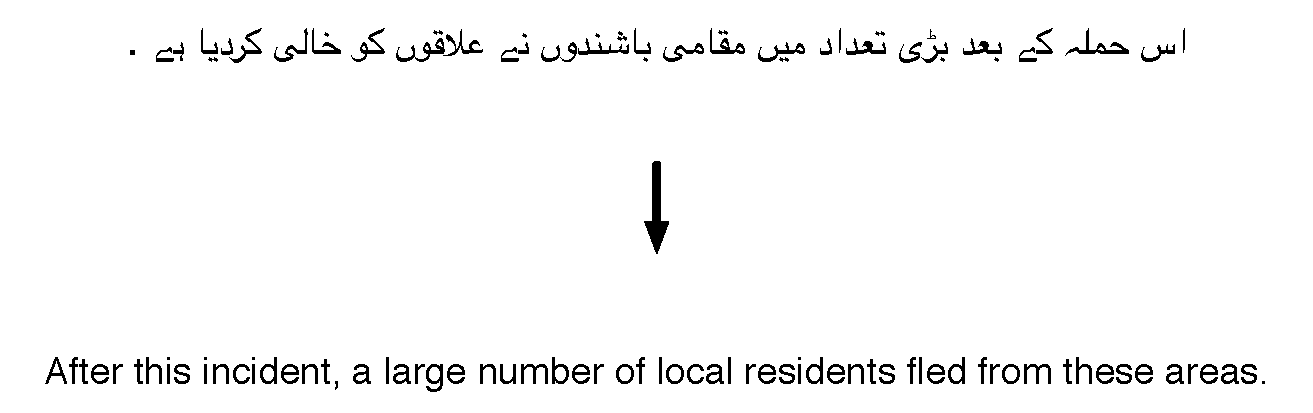
\includegraphics[scale=0.55]{urdu-ref.pdf}}
  \end{figure}
\end{exampleblock}
\begin{itemize}
  \item Statistical machine translation: Learn how to translate from parallel corpora 
\end{itemize}
\end{frame}

\begin{frame}[t]{Statistical machine translation: state-of-the-art}
%\vspace{1.0cm}
\begin{exampleblock}{Urdu $\rightarrow$ English}
  \begin{figure}
    {\centering 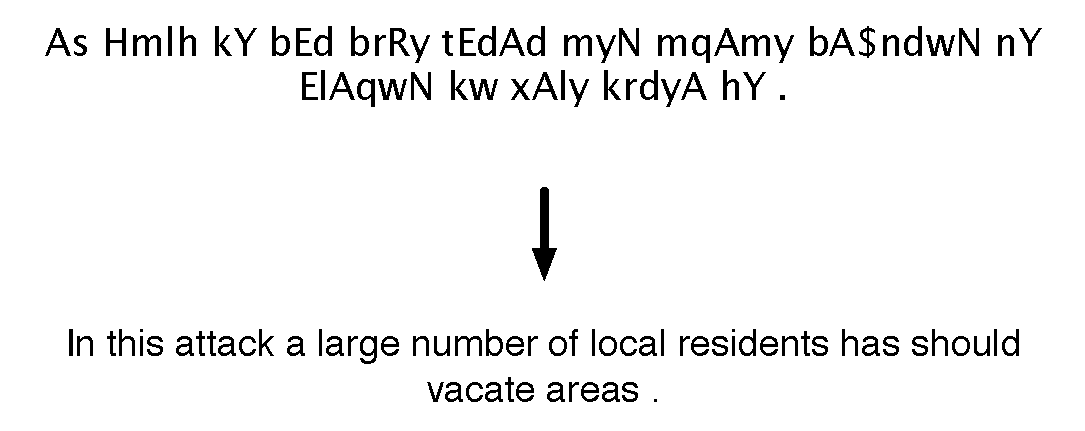
\includegraphics[scale=0.55]{urdu-bl.pdf}}
  \end{figure}
\end{exampleblock}
\begin{itemize}
  \item Current state-of-the-art translation models struggle with language pairs which exhibit large differences in structure.
\end{itemize}
\end{frame}


\begin{frame}[t]{Statistical machine translation: limitations}
\vspace{1.0cm}
\begin{exampleblock}{Structural divergence between languages:}
  %\vspace{0.3cm}
  \begin{table}
  \centering
    \only<1>{
    \begin{tabular}{|l|l|}
    \hline
      {\bf English}  & {\bf Who wrote this letter?} \\
      \hline
      Arabic   & \begin{Geeza}من الذي كتب هذه الرسالة؟\end{Geeza} \\
               & \textcolor{gray}{(function-word)} (who) (wrote) (this) (the-letter) \\
      \hline
      Chinese  & \begin{CJK}这封  信  是  谁  写  的 ?\end{CJK} \\
               & (this) (letter) (be) (who) (write) (come-from) \textcolor{gray}{(function-word)} \\
      \hline
    \end{tabular}
    }
    \only<2>{
    \begin{tabular}{|l|l|}
    \hline
      {\bf English}  & {\bf \textcolor{blue}{Who} \textcolor{green}{wrote} \textcolor{red}{this} \textcolor{orange}{letter?}} \\
      \hline
      Arabic   & \begin{Geeza}من الذي كتب هذه الرسالة؟\end{Geeza} \\
               & \textcolor{gray}{(function-word)} \textcolor{blue}{(who)} \textcolor{green}{(wrote)} \textcolor{red}{(this)} \textcolor{orange}{(the-letter)} \\
      \hline
      Chinese  & \begin{CJK}这封  信  是  谁  写  的 ?\end{CJK} \\
               & (this) (letter) (be) (who) (write) (come-from) \textcolor{gray}{(function-word)} \\
      \hline
    \end{tabular}
    }
    \only<3->{
    \begin{tabular}{|l|l|}
    \hline
      {\bf English}  & {\bf \textcolor{blue}{Who wrote} \textcolor{red}{this letter}?} \\
      \hline
      Arabic   & \begin{Geeza}من الذي كتب هذه الرسالة؟\end{Geeza} \\
               & \textcolor{gray}{(function-word)} (who) (wrote) (this) (the-letter) \\
      \hline
      Chinese  & \begin{CJK}\textcolor{red}{这封  信}  \textcolor{blue}{是  谁  写}  的 ?\end{CJK} \\
               & \textcolor{red}{(this) (letter)} \textcolor{blue}{(be) (who) (write) (come-from)} \textcolor{gray}{(function-word)} \\
      \hline
    \end{tabular}
  }
  \end{table}
\end{exampleblock}
\only<4>{
  \begin{itemize}
  \item Phrasal translation equivalences
  \item Constituent reordering
  \item Morphology
  \end{itemize}
}
\end{frame}

\begin{frame}[t]{Statistical machine translation: successes}
\begin{center}
  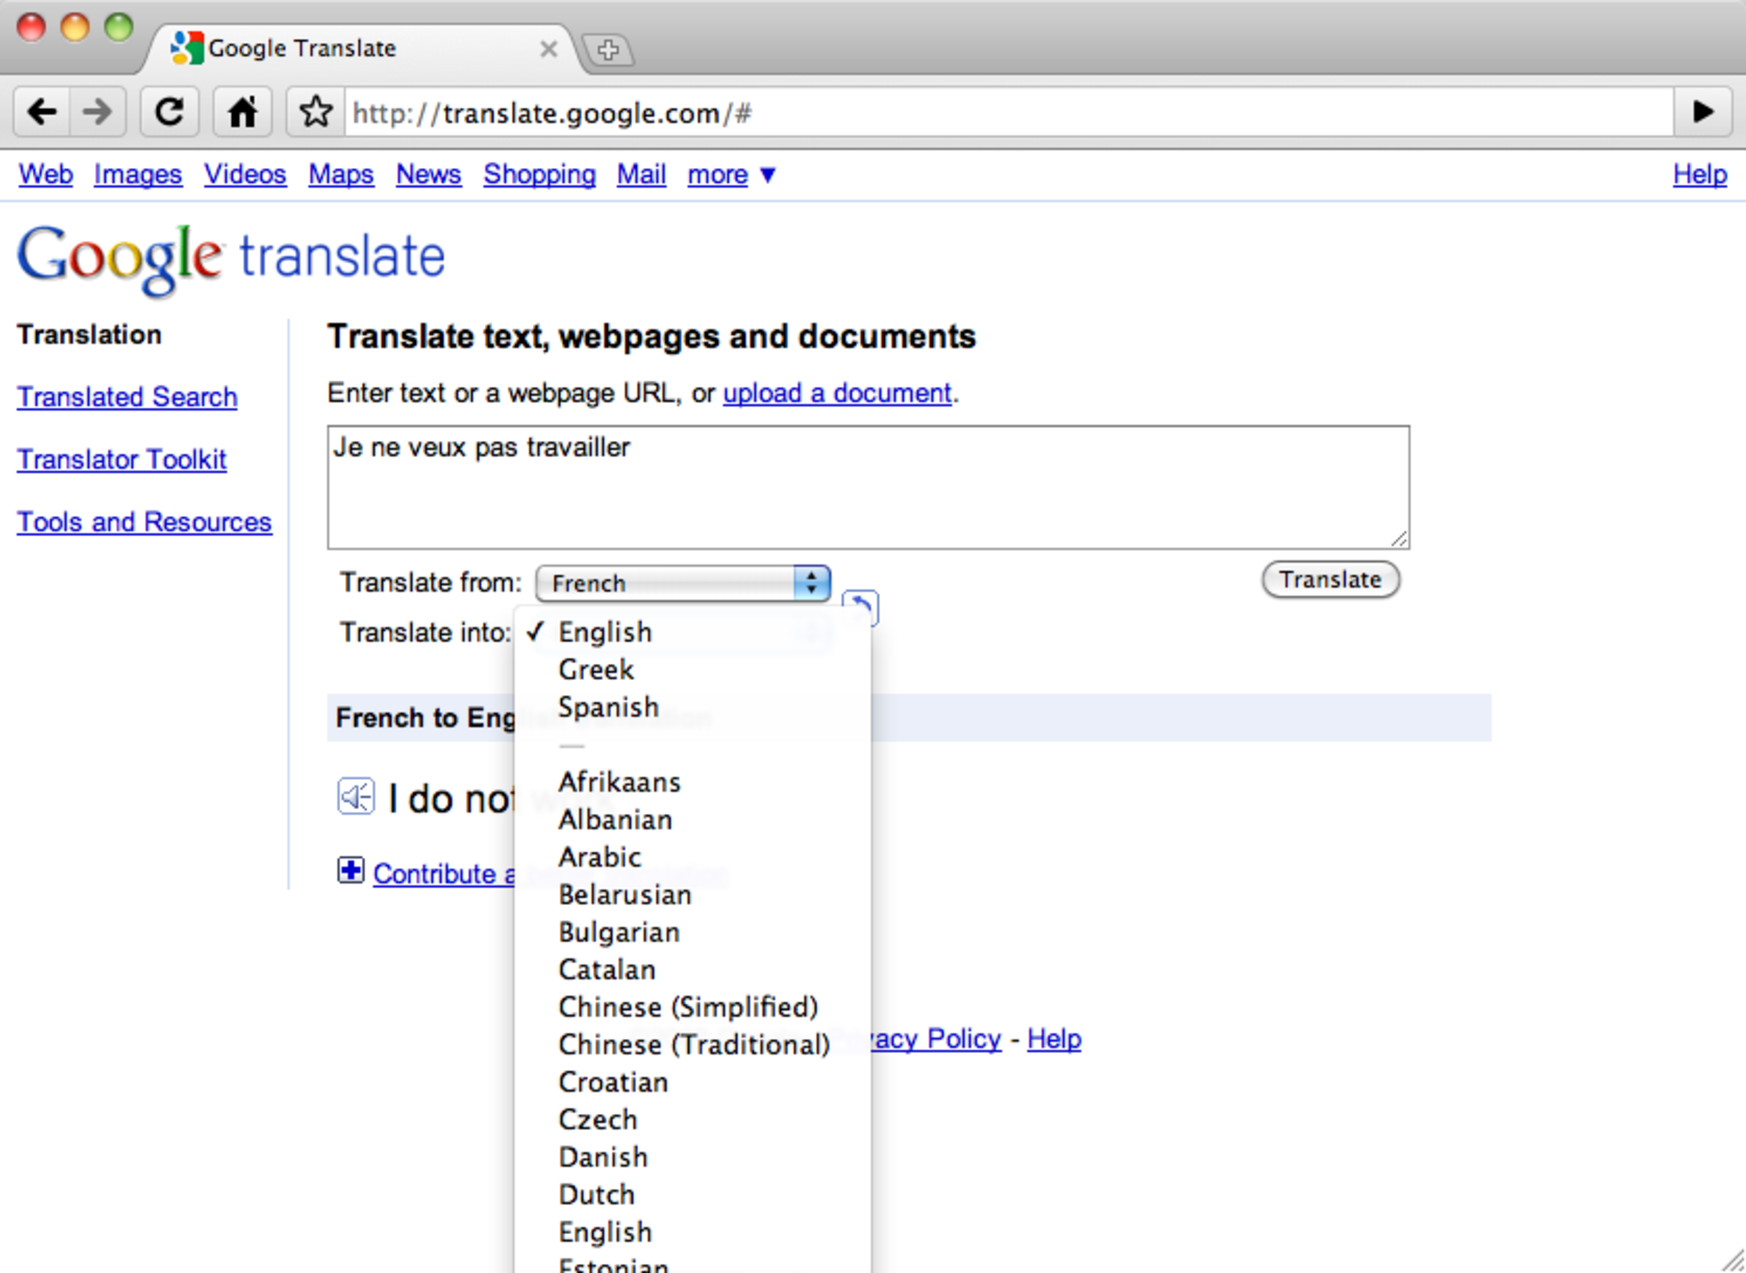
\includegraphics[scale=0.35]{GoogleTranslateLanguages.pdf}
\end{center}
\end{frame}

\begin{frame}
\frametitle{Using syntax in Machine Translation:}
  \footnotesize
  \begin{block}{Synchronous Context Free Grammar (SCFG)}
    \begin{figure}
    \begin{align*}
        \alert<2>{S} & \alert<2>{\rightarrow  \langle X\ind{1},\ X\ind{1} \rangle} 
            &\quad \alert<3,5>{X} & \alert<3,5>{\rightarrow  \langle X\ind{1}\ X\ind{2},\ X\ind{1}\ X\ind{2} \rangle} \\
        \alert<7>{X} & \alert<7>{\rightarrow  \langle X\ind{1}\ X\ind{2},\ X\ind{2}\ X\ind{1} \rangle} & &\\
        \alert<4>{X} & \alert<4>{\rightarrow  \langle Sie,\ She \rangle} 
           &\quad \alert<6>{X} & \alert<6>{\rightarrow  \langle will,\ wants\ to \rangle} \\
         \alert<8>{X} & \alert<8>{\rightarrow  \langle eine\ Tasse\ Kaffee,\ a\ cup\ of\ coffee \rangle}
           &\quad \alert<9>{X} & \alert<9>{\rightarrow  \langle trinken,\ drink\rangle} \\
    \end{align*}
    \end{figure}
  \end{block}
  \begin{exampleblock}{Example Derivation}
      %\begin{figure}
      %\begin{align*}
      \center
        \vspace{0.2cm}
        \onslide<2->{\alert<2>{$S \Rightarrow \langle X\ind{1},\ X\ind{1}\ \rangle$}} \quad \onslide<3->{\alert<3>{$\Rightarrow \langle X\ind{2}\ X\ind{3},\ X\ind{2}\ X\ind{3} \rangle$ \\}}
        \vspace{0.2cm}
        \onslide<4->{\alert<4>{$\Rightarrow \langle Sie\ X\ind{3},\ She\ X\ind{3} \rangle$}} \quad \onslide<5->{\alert<5>{$\Rightarrow \langle Sie\ X\ind{4}\ X\ind{5},\ She\ X\ind{4}\ X\ind{5} \rangle$ \\}}
        \vspace{0.2cm}
        \onslide<6->{\alert<6>{$\Rightarrow \langle Sie\ will\ X\ind{5},\ She\ wants\ to\  X\ind{5} \rangle$ }} \quad \onslide<7->{\alert<7>{$\Rightarrow \langle Sie\ will\ X\ind{6} X\ind{7},\ She\ wants\ to\  X\ind{7} X\ind{6} \rangle$ \\}}
        \vspace{0.2cm}
        \onslide<8->{\alert<8>{$\Rightarrow \langle Sie\ will\ eine\ Tasse\ Kaffee\ X\ind{7},\ She\ wants\ to\ X\ind{7}\ a\ cup\ of\ coffee\rangle$} \\}
        \vspace{0.2cm}
        \onslide<9->{\alert<9>{$\Rightarrow \langle Sie\ will\ eine\ Tasse\ Kaffee\ trinken,\ She\ wants\ to\ drink\ a\ cup\ of\ coffee\rangle$}}
        \vspace{0.2cm}
      %\end{align*}
      %\end{figure}
  \end{exampleblock}
\end{frame}


\begin{frame}[t]{Models of translation}
\begin{block}{Unlabelled SCFG: Hiero}
  \begin{center}
    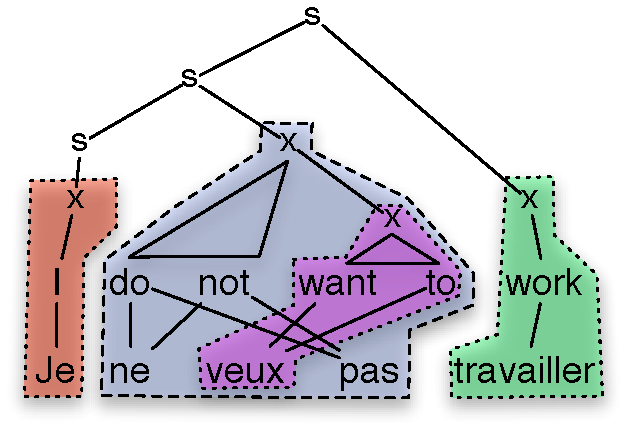
\includegraphics[scale=0.55]{JeNeVeuxPasTravailler-Hiero.pdf}
    \hspace{0.3in}
    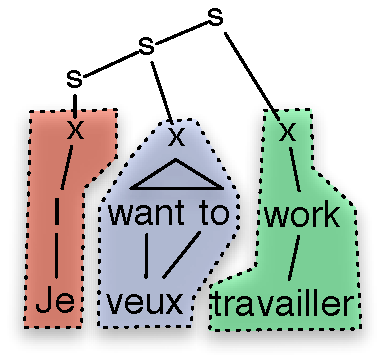
\includegraphics[scale=0.55]{JeVeuxTravailler-Hiero.pdf}
  \end{center}
\end{block}
\begin{itemize}
\item Only requires the parallel corpus.
\item But weak model of sentence structure.
\end{itemize}
\end{frame}

\begin{frame}[t]{Models of translation}
\begin{exampleblock}{Supervised SCFG: Syntactic Tree-to-String}
\begin{center}
  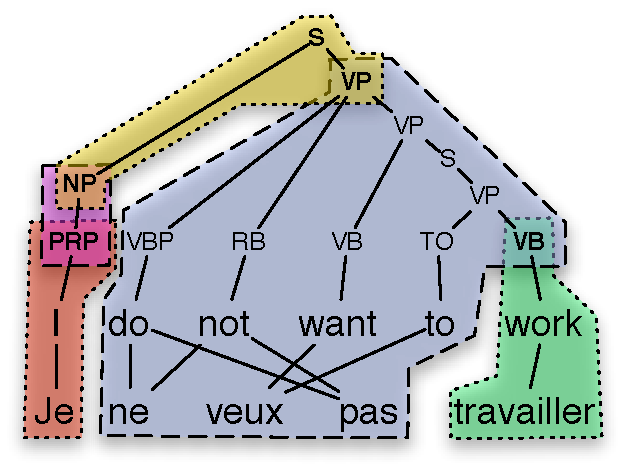
\includegraphics[scale=0.55]{JeNeVeuxPasTravailler-tsg.pdf}
  \hspace{0.3in}
  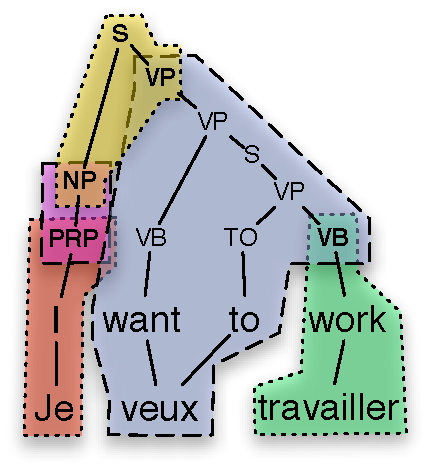
\includegraphics[scale=0.55]{JeVeuxTravailler-tsg.pdf}
\end{center}
\end{exampleblock}
\begin{itemize}
\item Strong model of sentence structure.
\item Reliant on a treebank to train the parser.
\end{itemize}
\end{frame}


\begin{frame}[t]{Impact}
\vspace{0.5in}
\begin{table}
  \begin{tabular}{l|rr}
    \hline
    Language & Words &  Domain \\ \hline
    English & 4.5M& Financial news \\
    Chinese & 0.5M & Broadcasting news \\ 
    Arabic &  300K (1M planned)  &  News  \\
    Korean & 54K  & Military \\ \hline
  \end{tabular}
\caption{Major treebanks: data size and domain \label{table_treebanks_size}}
\end{table}
\end{frame}


\begin{frame}[t]{Impact}
Parallel corpora far exceed treebanks (millions of words):
  \begin{figure}
    {\centering 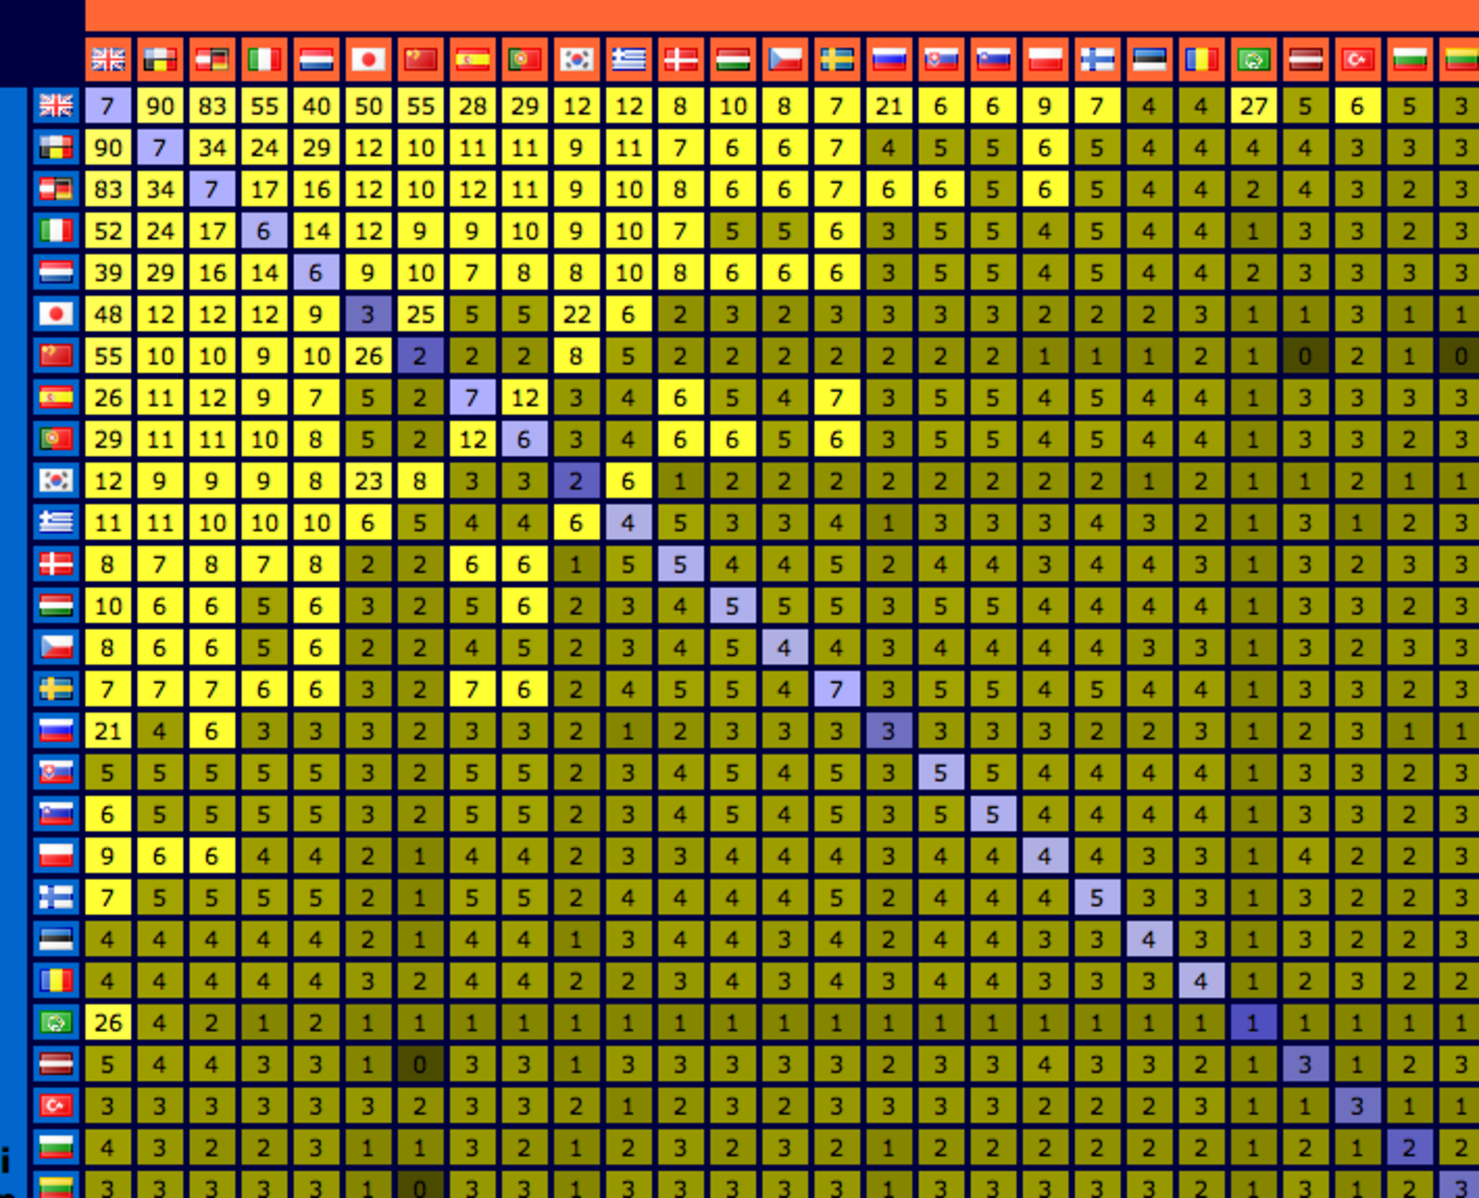
\includegraphics[scale=0.7]{resource_matrix.pdf}}
  \end{figure}
\end{frame}


\begin{frame}[t]{Models of translation}
\begin{exampleblock}{Phrase extraction:}
\begin{center}
\only<1>{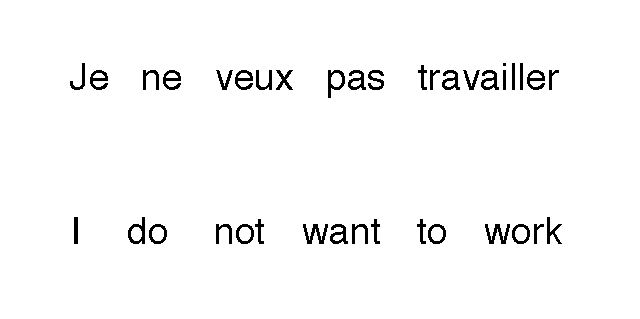
\includegraphics[scale=0.8]{PhraseExtraction6.pdf}\\[1cm]}
\only<2>{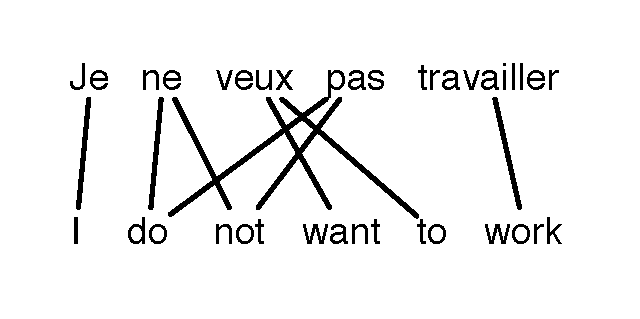
\includegraphics[scale=0.8]{PhraseExtraction5.pdf}\\[1cm]}
\only<3>{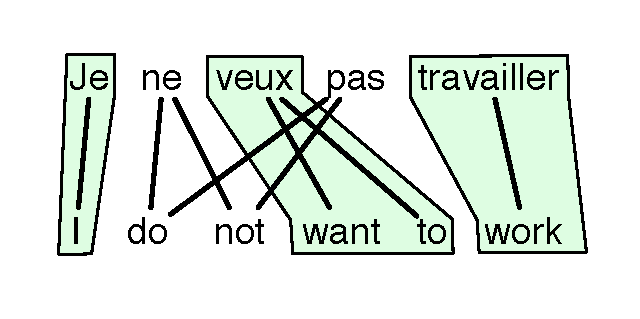
\includegraphics[scale=0.8]{PhraseExtraction4.pdf}\\[1cm]}
\only<4>{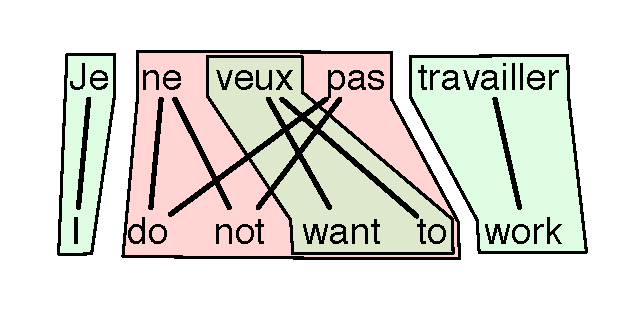
\includegraphics[scale=0.8]{PhraseExtraction3.pdf}\\[1cm]}
\only<5>{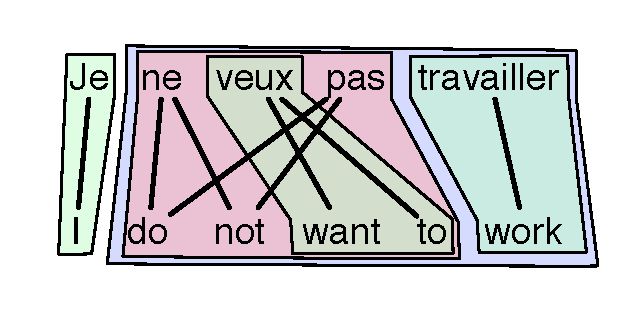
\includegraphics[scale=0.8]{PhraseExtraction2.pdf}\\[1cm]}
\only<6>{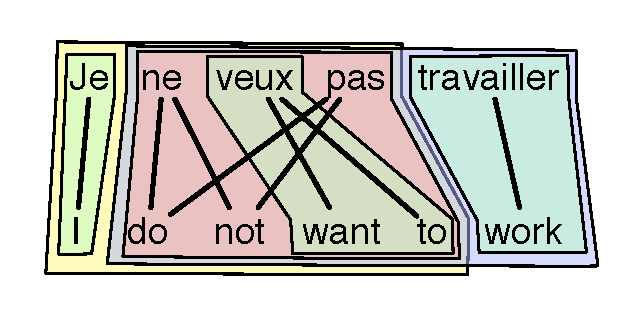
\includegraphics[scale=0.8]{PhraseExtraction1.pdf}\\[1cm]}
\only<7>{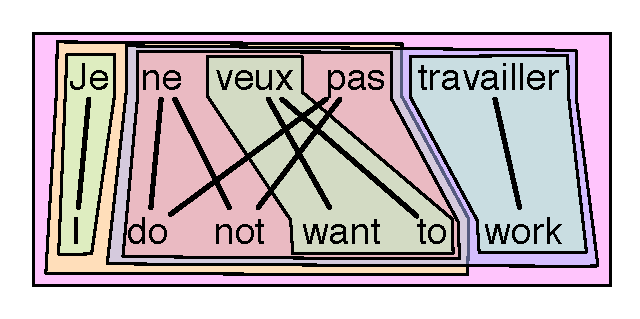
\includegraphics[scale=0.8]{PhraseExtraction.pdf}\\[1cm]}
\end{center}
\end{exampleblock}
\only<2->{
\begin{unpacked_itemize}
\only<2>{\item Use a word-based translation model to annotate the parallel corpus with word-alignments}
\only<3->{\item $\langle$ Je, I $\rangle$, $\langle$ veux, want to $\rangle$,  $\langle$ travailler, work $\rangle$}\only<4->{, $\langle$ ne veux pas, do not want to $\rangle$}\only<5->{, $\langle$ ne veux pas travailler, do not want to work $\rangle$}\only<6->{, $\langle$ Je ne veux pas, I do not want to $\rangle$}\only<7->{, $\langle$ Je ne veux pas travailler, I do not want to work $\rangle$}
\end{unpacked_itemize}
}
\end{frame}


\begin{frame}[t]{Models of translation}
\begin{exampleblock}{SCFG Rule extraction:}
\begin{center}
\only<1>{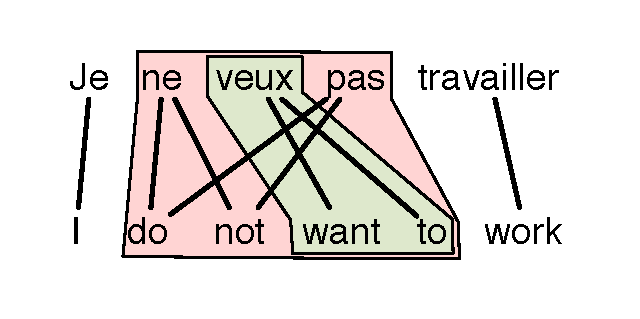
\includegraphics[scale=0.8]{HieroExtraction1.pdf}\\[1cm]}
\only<2>{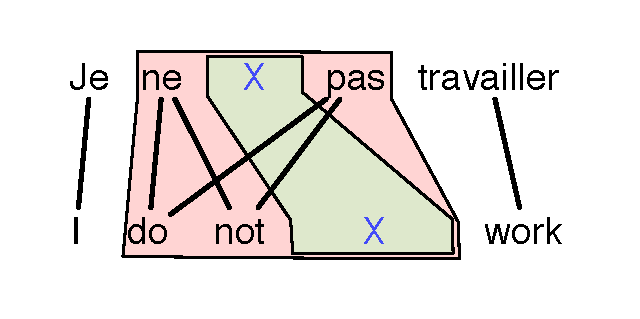
\includegraphics[scale=0.8]{HieroExtraction2.pdf}\\[1cm]}
\only<3>{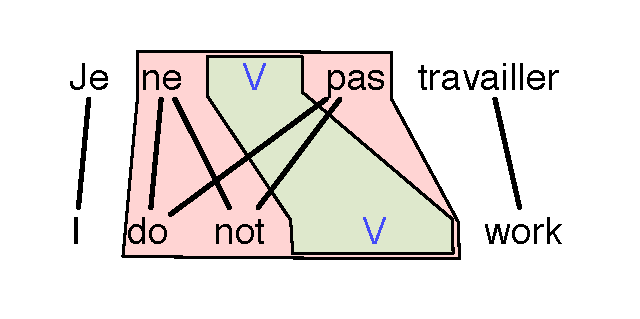
\includegraphics[scale=0.8]{HieroExtraction3.pdf}\\[1cm]}
\only<4>{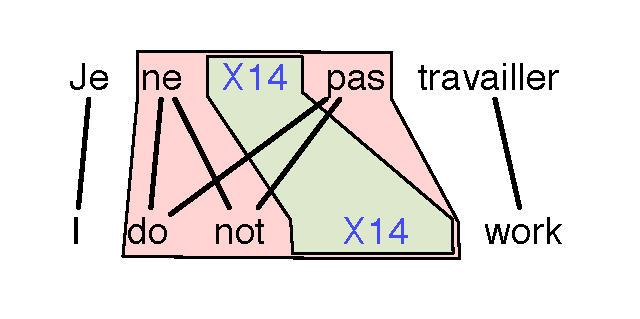
\includegraphics[scale=0.8]{HieroExtraction4.pdf}\\[1cm]}
\end{center}
\end{exampleblock}
\begin{unpacked_itemize}
\only<1>{ \item X -> $\langle$ ne veux pas, do not want to $\rangle$ }
\only<2>{ \item X -> $\langle$ ne veux pas, do not want to $\rangle$, \item X -> $\langle$ ne X\ind{1} pas, do not X\ind{1} $\rangle$ }
\only<3>{ \item VP$/$NN -> $\langle$ ne veux pas, do not want to $\rangle$, \item VP$/$NN -> $\langle$ ne V\ind{1} pas, do not V\ind{1} $\rangle$ }
\only<4>{ \item X10 -> $\langle$ ne veux pas, do not want to $\rangle$, \item X10 -> $\langle$ ne X14\ind{1} pas, do not X14\ind{1} $\rangle$ }
\end{unpacked_itemize}
\end{frame}

\begin{frame}[t]{Workshop overview}
Input:
  \begin{itemize}
%  \item Joshua decoder
  \item Existing procedures for unlabelled synchronous grammar extraction
  \end{itemize}
\vspace{0.3in}
Output:
  \begin{itemize}
    \item New unsupervised models for large scale synchronous grammar extraction,
%    \item An implementation of this model,
    \item A comparison and analysis of the existing and proposed models,
    \item Extended decoders (cdec/Joshua) capable of working efficiently with these models.
  \end{itemize}
\end{frame}


%\begin{frame}[t]{Models of translation}
%\begin{block}{Hierarchical}
%  \begin{center}
%    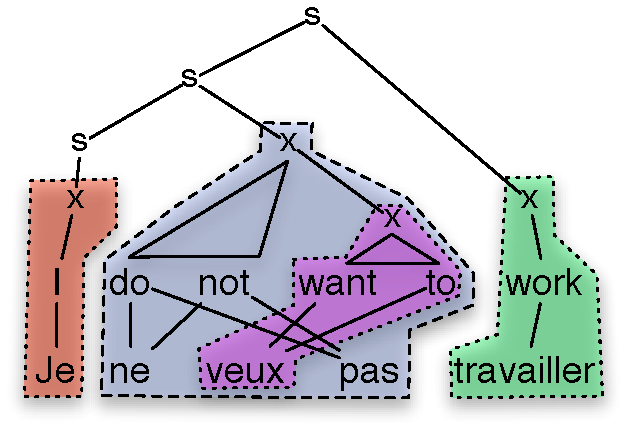
\includegraphics[scale=0.55]{JeNeVeuxPasTravailler-Hiero.pdf}
%    \hspace{0.3in}
%    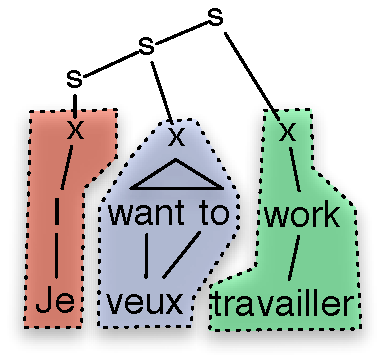
\includegraphics[scale=0.55]{JeVeuxTravailler-Hiero.pdf}
%  \end{center}
%\end{block}
%\end{frame}


%\begin{frame}[t]{Impact}
%  \begin{center}
%    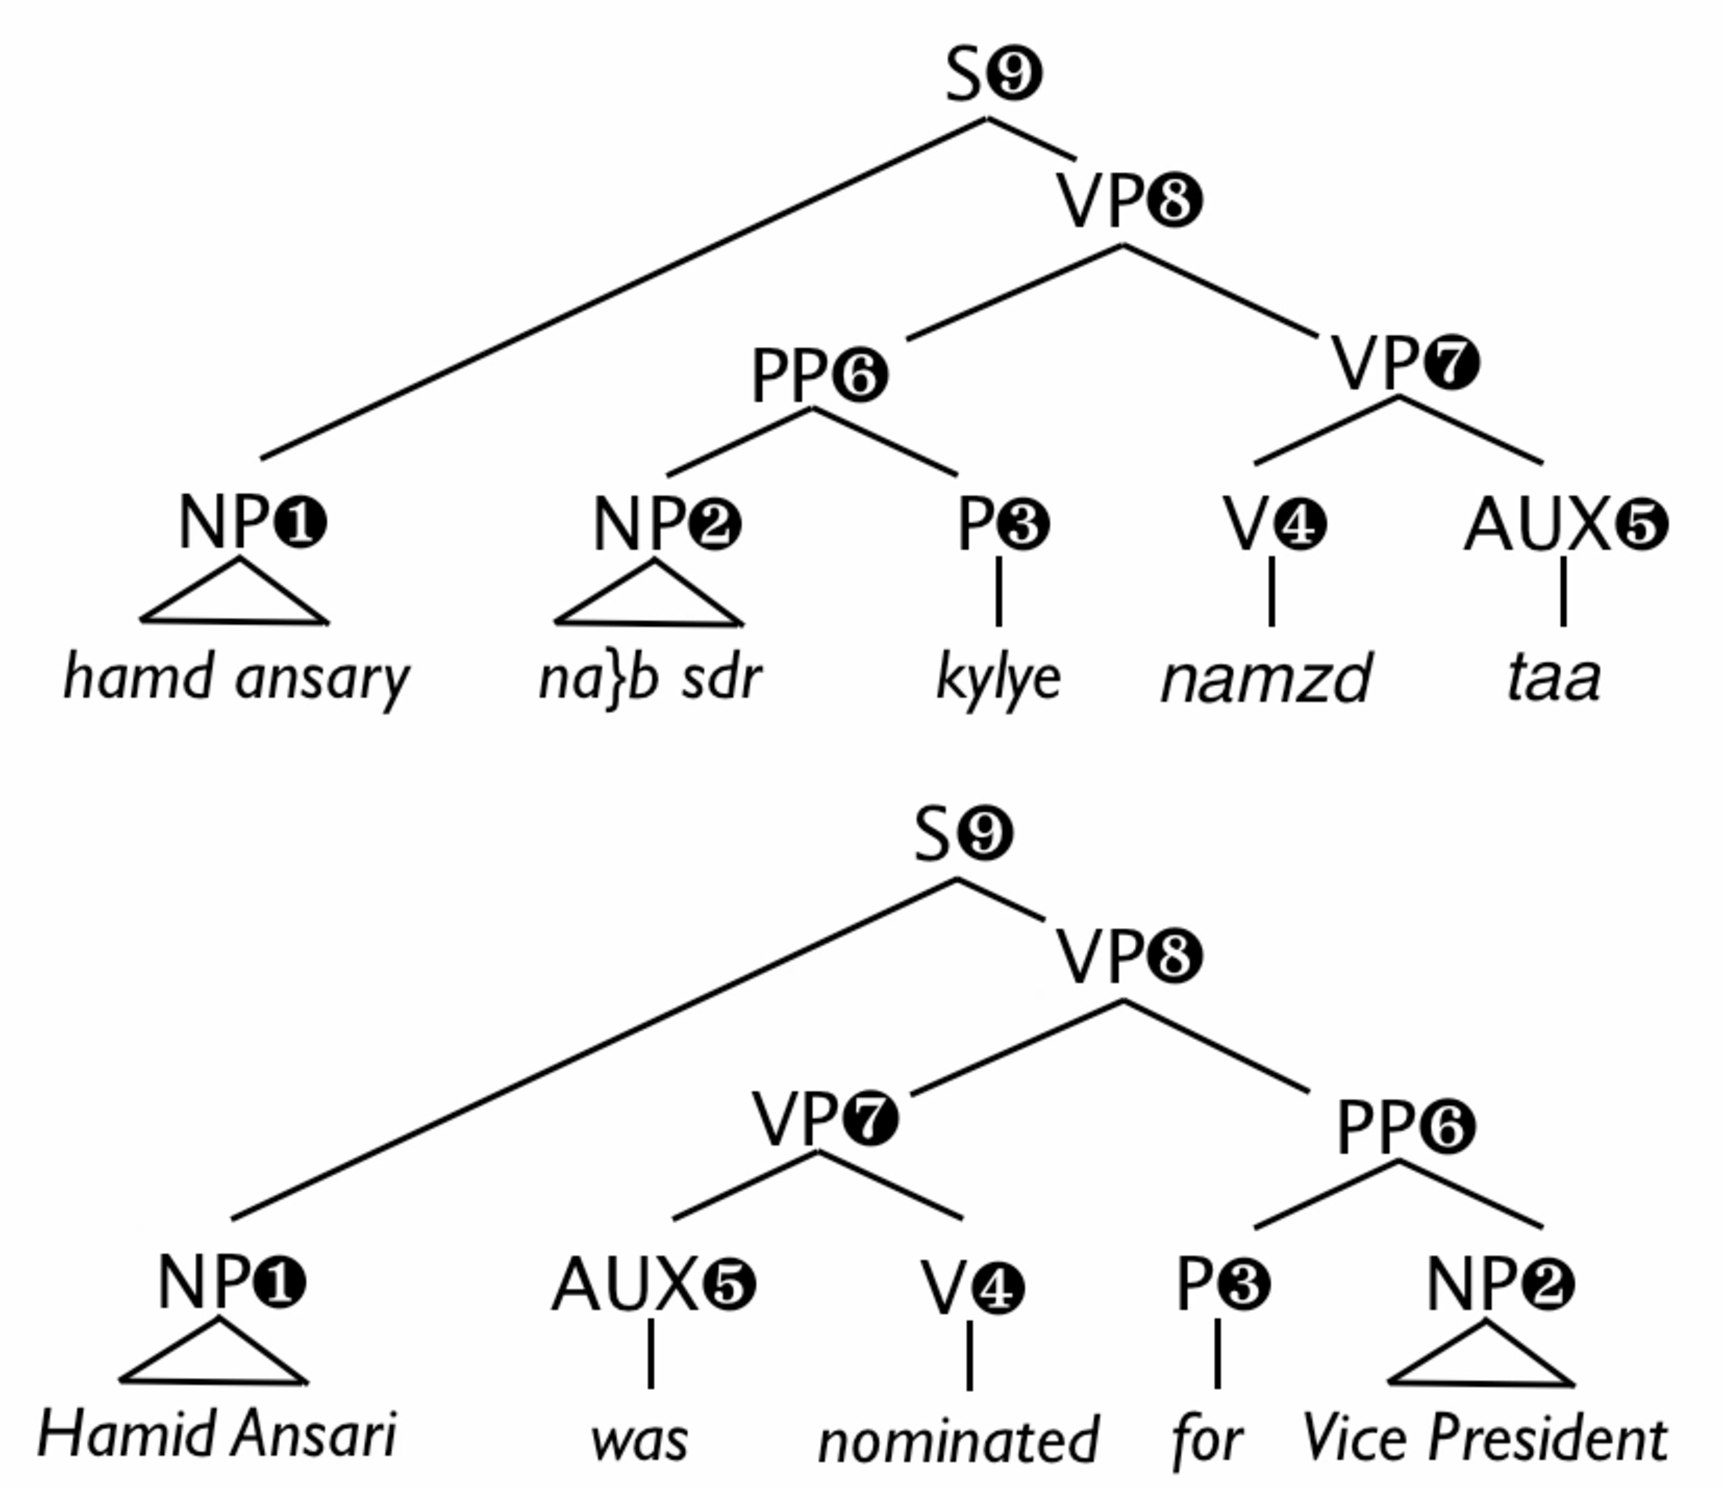
\includegraphics[scale=0.3]{ccb_tree.pdf}
%  \end{center}
%\end{frame}



%\begin{frame}[t]{Models of translation}
%\vspace{0.25in}
%\begin{block}{Hierarchical}
%  \begin{center}
%    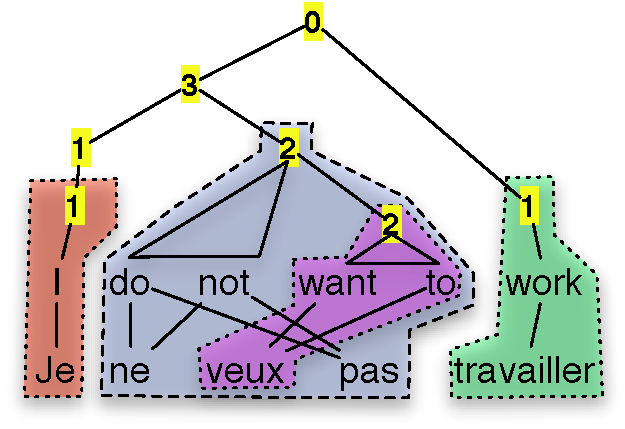
\includegraphics[scale=0.55]{JeNeVeuxPasTravailler-Hiero-labelled.pdf}
%    \hspace{0.3in}
%    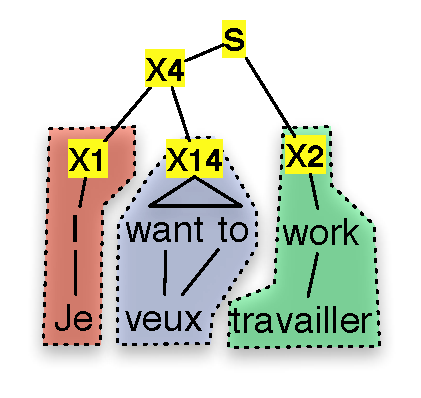
\includegraphics[scale=0.55]{JeVeuxTravailler-Hiero-labelled.pdf}
%  \end{center}
%\end{block}
%%\begin{itemize}
%%\item \alert{AIM: Implement a large scale open-source synchronous constituent learning system.} 
%%\item \alert{AIM: Investigate and understand the relationship between the choice of synchronous grammar and SMT performance,} 
%%\item \alert{AIM: and fix our decoders accordingly.} 
%%\end{itemize}
%\end{frame}
%
%\begin{frame}[t]{Evaluation goals}
%We will predominately evaluate using BLEU, but also use automatic structured metrics and perform small scale human evaluation:
%\vspace{0.25in}
%\begin{unpacked_itemize}
%\item Evaluate phrasal, syntactic, unsupervised syntactic,
%\item Aim 1: Do no harm (not true of existing syntactic approach)
%\item Aim 2: Exceed the performance of current non-syntactic systems.
%\item Aim 3: Meet or exceed performance of existing syntactic systems.
%\end{unpacked_itemize}
%\end{frame}

%\begin{frame}[t]{Impact}
%Success will have a significant impact on two areas of CL:
%\vspace{0.25in}
%\begin{unpacked_itemize}
%\item Machine translation
%\begin{unpacked_itemize}
%  \item Make the benefits of richly structured translation models available to a much wider range of researchers and for a wider range of languages.
%% \item Change the research outlook of the field.
%\end{unpacked_itemize}
%\item Grammar induction:
%\begin{unpacked_itemize}
%  \item Provide an empirical validation of state-of-the-art grammar induction techniques.
%\end{unpacked_itemize}
%\end{unpacked_itemize}
%\end{frame}


\begin{frame}[t]{Workshop Streams}
Expand, describing challenges faced in each stream.
\vspace{0.25in}
\begin{unpacked_itemize}
\item Implement scalable SCFG grammar extraction algorithms.
\item Improve SCFG decoders to efficiently handle the grammars produce.
\item Investigate discriminative training regimes to leverage features extracted from these grammars.
\end{unpacked_itemize}
\end{frame}

\begin{frame}[t]{Extrinsic evaluation: Bleu}
\begin{exampleblock}{
   \only<1>{Ngram overlap metrics:}
   \only<2>{Ngram overlap metrics: 1-gram precision $p_1 = \frac{11}{14}$}
   \only<3>{Ngram overlap metrics: 2-gram precision $p_2 = \frac{5}{13}$}
   \only<4>{Ngram overlap metrics: 3-gram precision $p_3 = \frac{2}{12}$}
   \only<5>{Ngram overlap metrics: 4-gram precision $p_4 = \frac{1}{11}$}
}
\vspace{0.2cm}
{\em Source}: \begin{CJK}欧盟 办事处 与 澳洲 大使馆 在 同 一 建筑 内 \end{CJK} \\
\vspace{0.3cm}
\only<1>{{\em Candidate}: the chinese embassy in australia and the eu representative office in the same building}
\only<2>{{\em Candidate}: \alert{the} chinese \alert{embassy} \alert{in} australia \alert{and} \alert{the} \alert{eu} representative \alert{office} \alert{in} \alert{the} \alert{same} \alert{building}}
\only<3>{{\em Candidate}: the chinese embassy in australia \alert{and} \alert{the} \alert{eu} representative office \alert{in} \alert{the} \alert{same} \alert{building}}
\only<4>{{\em Candidate}: the chinese embassy in australia and the eu representative office \alert{in} \alert{the} \alert{same} \alert{building}}
\only<5>{{\em Candidate}: the chinese embassy in australia and the eu representative office \alert{in} \alert{the} \alert{same} \alert{building}}
\vspace{0.2cm}
\end{exampleblock}

\begin{block}{Reference Translations:}
  \begin{enumerate}
  \only<1>{\item the eu office and the australian embassy are housed in the same building}
  \only<2>{\item \alert{the} \alert{eu} \alert{office} \alert{and} \alert{the} australian \alert{embassy} are housed \alert{in} \alert{the} \alert{same} \alert{building}}
  \only<3>{\item \alert{the} \alert{eu} office \alert{and} \alert{the} australian embassy are housed \alert{in} \alert{the} \alert{same} \alert{building}}
  \only<4>{\item the eu office and the australian embassy are housed \alert{in} \alert{the} \alert{same} \alert{building}}
  \only<5>{\item the eu office and the australian embassy are housed \alert{in} \alert{the} \alert{same} \alert{building}}

  \only<1>{\item the european union office is in the same building as the australian embassy}
  \only<2>{\item \alert{the} european union \alert{office} is \alert{in} \alert{the} \alert{same} \alert{building} as \alert{the} australian \alert{embassy}}
  \only<3>{\item the european union office is \alert{in} \alert{the} \alert{same} \alert{building} as the australian embassy}
  \only<4>{\item the european union office is \alert{in} \alert{the} \alert{same} \alert{building} as the australian embassy}
  \only<5>{\item the european union office is \alert{in} \alert{the} \alert{same} \alert{building} as the australian embassy}

  \only<1>{\item the european union 's office and the australian embassy are both located in the same building}
  \only<2>{\item \alert{the} european union 's \alert{office} \alert{and} \alert{the} australian \alert{embassy} are both located \alert{in} \alert{the} \alert{same} \alert{building}}
  \only<3>{\item the european union 's office \alert{and} \alert{the} australian embassy are both located \alert{in} \alert{the} \alert{same} \alert{building}}
  \only<4>{\item the european union 's office and the australian embassy are both located \alert{in} \alert{the} \alert{same} \alert{building}}
  \only<5>{\item the european union 's office and the australian embassy are both located \alert{in} \alert{the} \alert{same} \alert{building}}
  
  \only<1>{\item the eu 's mission is in the same building with the australian embassy}
  \only<2>{\item \alert{the} \alert{eu} 's mission is \alert{in} \alert{the} \alert{same} \alert{building} with \alert{the} australian \alert{embassy}}
  \only<3>{\item \alert{the} \alert{eu} 's mission is \alert{in} \alert{the} \alert{same} \alert{building} with the australian embassy}
  \only<4>{\item the eu 's mission is \alert{in} \alert{the} \alert{same} \alert{building} with the australian embassy}
  \only<5>{\item the eu 's mission is \alert{in} \alert{the} \alert{same} \alert{building} with the australian embassy}
  \end{enumerate}
\end{block}
\end{frame}

\begin{frame}[t]{Extrinsic evaluation: Bleu}
\begin{exampleblock}{BLEU}
\Large
\begin{align}
\nonumber BLEU_n = BP \times \exp{\left( \sum_{n=1}^{N} w_n \log{p_n} \right) }\\
\nonumber BP = \left\{ 
  \begin{array}{ll} 
    1 & \mbox{if $c > r$}  \\
    \exp{(1-\frac{R'}{C'})} & \mbox{if $c <= r$}
  \end{array} \right.
\end{align}
\end{exampleblock}
\begin{itemize}
\item {\em BP} is the {\em Brevity Penalty}, $w_n$ is the ngram length weights (usually $\frac{1}{n}$), $p_n$ is precision of ngram predictions, $R'$ is the total length of all references and $C'$ is the sum of the best matching candidates.
\item statistics are calculate over the whole {\em document}, i.e. all the sentences.
\end{itemize}
\end{frame}



\begin{frame}[t]{Language pairs}
\begin{unpacked_itemize}
\item BTEC Chinese-English:
  \begin{itemize}
  \item 44k sentence pairs, short sentences
  \item Widely reported `prototyping' corpus
  \item Hiero baseline score: 57.0 (16 references)
  \end{itemize}
\item NIST Urdu-English:
  \begin{itemize}
  \item 50k sentence pairs
  \item Hiero baseline score: 21.1 (4 references)
  \item Major challenges: major long-range reordering, SOV word order
  \end{itemize}
\item Europarl Dutch-French:
  \begin{itemize}
  \item 100k sentence pairs, standard Europarl test sets
  \item Hiero baseline score: Europarl 2008 - 26.3 (1 reference)
  \item Major challenges: V2 / V-final word order, morphology
  \end{itemize}
\end{unpacked_itemize}
\end{frame}


\begin{frame}[t]{Outline}
\begin{columns}
  \begin{column}{0.2\textwidth}
    \begin{exampleblock}{}
      \begin{figure}
        \tiny
        {\centering 
\includegraphics[scale=0.07]{trevor.jpg}} \\
        Trevor Cohn \\
        
        {\centering 
\includegraphics[scale=0.06]{dyer.jpg}} \\
        Chris Dyer\\
        
        {\centering 
\includegraphics[scale=0.11]{jan.jpg}} \\
        Jan Botha \\
        
        {\centering 
\includegraphics[scale=0.06]{olivia.jpg}} \\
        Olivia Buzek\\
        
        {\centering 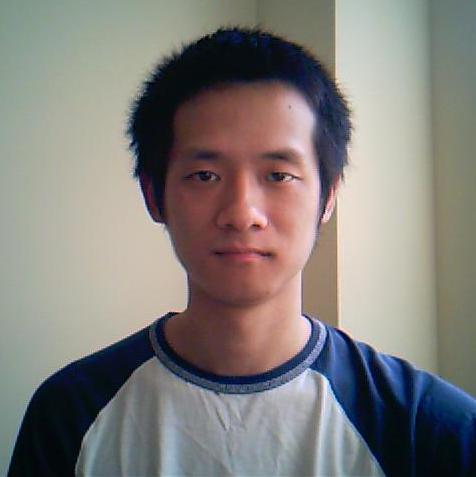
\includegraphics[scale=0.10]{desai.jpg}}\\
        Desai Chen\\

      \end{figure}
    \end{exampleblock}
  \vspace{0.25in}
  \end{column}
  \begin{column}{0.7\textwidth}
    \begin{unpacked_itemize}
      \item 1:55pm Experimental Setup. Trevor
      \item 2:10pm Non-parametric models of category induction. Chris
      \item 2:25pm Inducing categories for morphology. Jan
      \item 2:35pm Smoothing, backoff and hierarchical grammars. Olivia
      \item 2:45pm Parametric models: posterior regularisation. Desai
      \item 3:00pm Break.
    \end{unpacked_itemize}
  \end{column}
\end{columns}
\end{frame}



\begin{frame}[t]{Outline}
\begin{columns}
  \begin{column}{0.2\textwidth}
    \begin{exampleblock}{}
      \begin{figure}
        \tiny
        {\centering 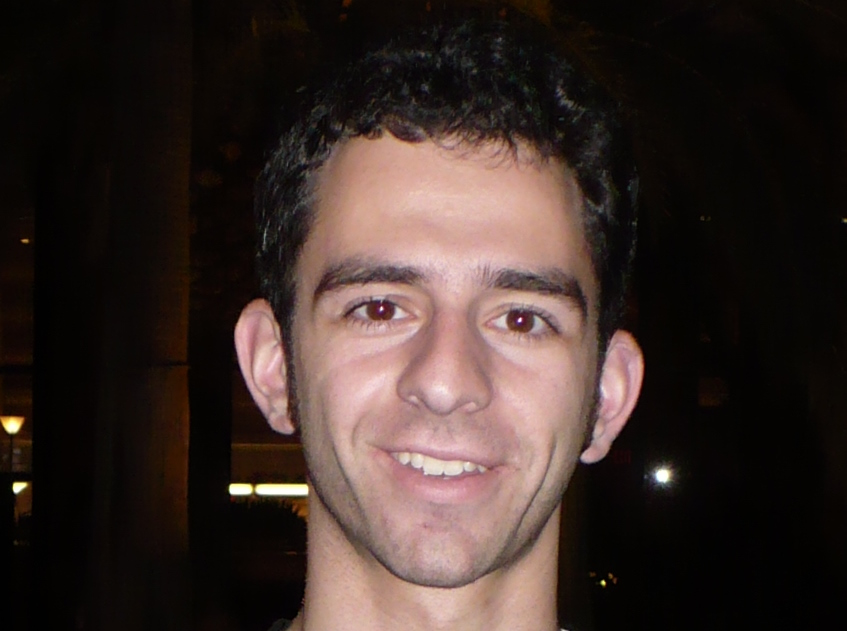
\includegraphics[scale=0.05]{vlad.jpg}} \\
        Vlad Eidelman\\
        
        {\centering 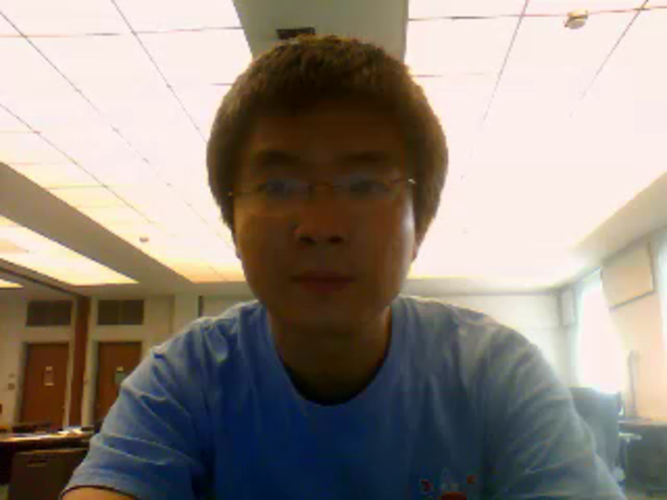
\includegraphics[scale=0.15]{ziyuan.pdf}} \\
        Ziyuan Wang\\
        
        {\centering 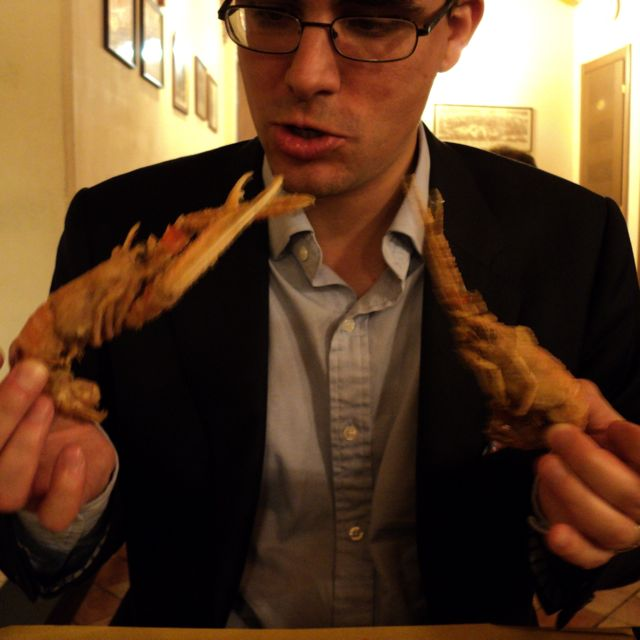
\includegraphics[scale=0.06]{adam.jpg}} \\
        Adam Lopez\\
        
        {\centering 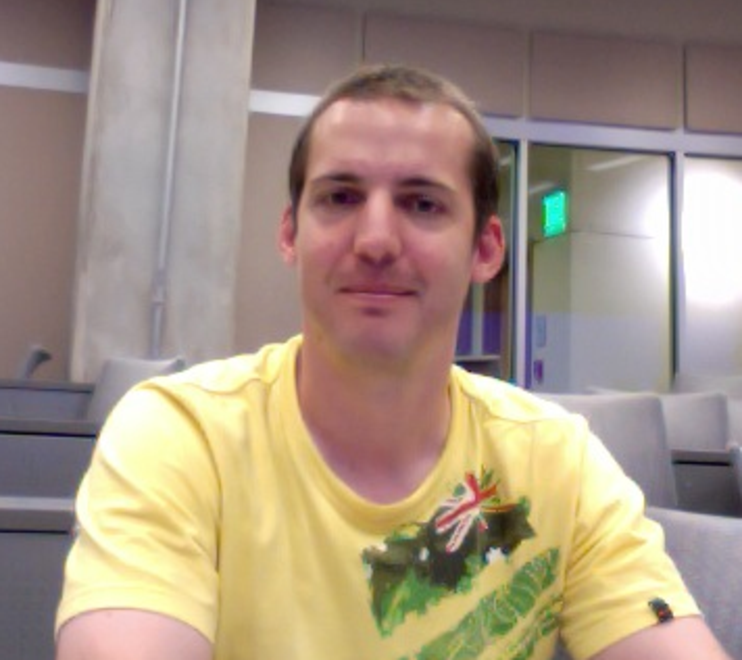
\includegraphics[scale=0.10]{jon.pdf}} \\
        Jon Graehl\\
        
        {\centering 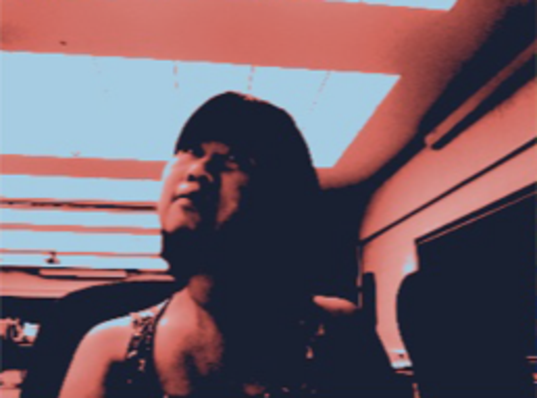
\includegraphics[scale=0.15]{linh.pdf}} \\
        ThuyLinh Nguyen\\

      \end{figure}
    \end{exampleblock}
  \vspace{0.25in}
  \end{column}
  \begin{column}{0.7\textwidth}
    \begin{itemize}
    \setlength{\itemsep}{25pt}
    \setlength{\parskip}{0pt}
    \setlength{\parsep}{0pt}
    \item 3:15pm Training models with rich features spaces. Vlad
    \item 3:30pm Decoding with complex grammars. Adam
    \item 4:00pm Closing remarks. Phil
    \item 4:05pm Finish.
    \end{itemize}
  \end{column}
\end{columns}
\end{frame}



\begin{frame}[t]{Remember:}
  \vspace{0.5in}
  \begin{unpacked_itemize}
    \item Idea: Learn synchronous grammar labels which encode substituteability; phrases which occur in the same context should receive the same label.
    \item Result: Better models of translation structure, morphology and improved decoding algorithms.
  \end{unpacked_itemize}
\end{frame}

\begin{frame}[t]{This slide is intentionally left blank.}
\end{frame}

\begin{frame}[t]{Outline}
\begin{columns}
  \begin{column}{0.2\textwidth}
    \begin{exampleblock}{}
      \begin{figure}
        \tiny
        {\centering 
\includegraphics[scale=0.07]{trevor.jpg}} \\
        Trevor Cohn \\
        
        {\centering 
\includegraphics[scale=0.06]{dyer.jpg}} \\
        Chris Dyer\\
        
        {\centering 
\includegraphics[scale=0.11]{jan.jpg}} \\
        Jan Botha \\
        
        {\centering 
\includegraphics[scale=0.06]{olivia.jpg}} \\
        Olivia Buzek\\
        
        {\centering 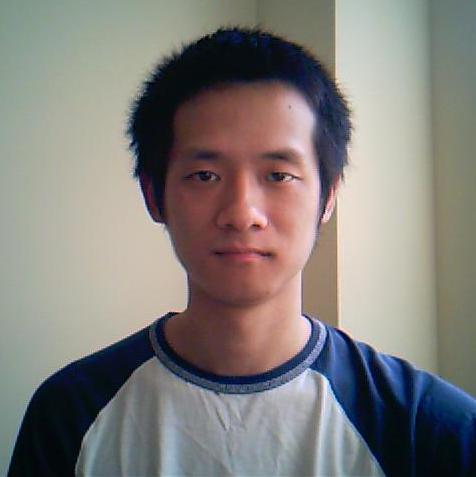
\includegraphics[scale=0.10]{desai.jpg}}\\
        Desai Chen\\

      \end{figure}
    \end{exampleblock}
  \vspace{0.25in}
  \end{column}
  \begin{column}{0.7\textwidth}
    \begin{unpacked_itemize}
      \only<1>{\item \alert{1:55pm Experimental Setup. Trevor}}
      \only<2->{\item 1:55pm Experimental Setup. Trevor}
      \only<2>{\item \alert{2:10pm Non-parametric models of category induction. Chris}}
      \only<1,3->{\item 2:10pm Non-parametric models of category induction. Chris}
      \only<3>{\item \alert{2:25pm Inducing categories for morphology. Jan}}
      \only<1,2,4->{\item 2:25pm Inducing categories for morphology. Jan}
      \only<4>{\item \alert{2:35pm Smoothing, backoff and hierarchical grammars. Olivia}}
      \only<1-3,5->{\item 2:35pm Smoothing, backoff and hierarchical grammars. Olivia}
      \only<5>{\item \alert{2:45pm Parametric models: posterior regularisation. Desai}}
      \only<1-4,6->{\item 2:45pm Parametric models: posterior regularisation. Desai}
      \only<6>{\item \alert{3:00pm Break.}}
      \only<1-5>{\item 3:00pm Break.}
    \end{unpacked_itemize}
  \end{column}
\end{columns}
\end{frame}



\begin{frame}[t]{Outline}
\begin{columns}
  \begin{column}{0.2\textwidth}
    \begin{exampleblock}{}
      \begin{figure}
        \tiny
        {\centering 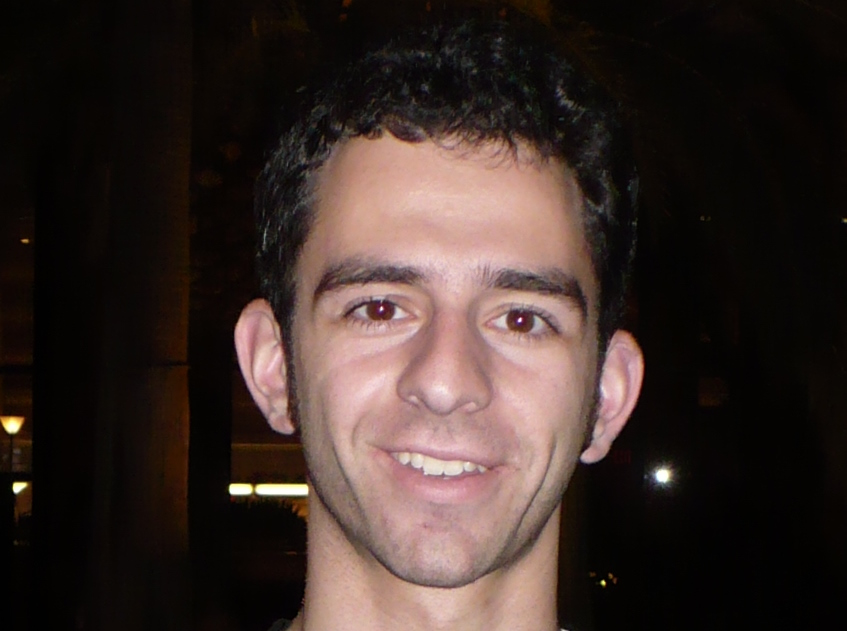
\includegraphics[scale=0.05]{vlad.jpg}} \\
        Vlad Eidelman\\
        
        {\centering 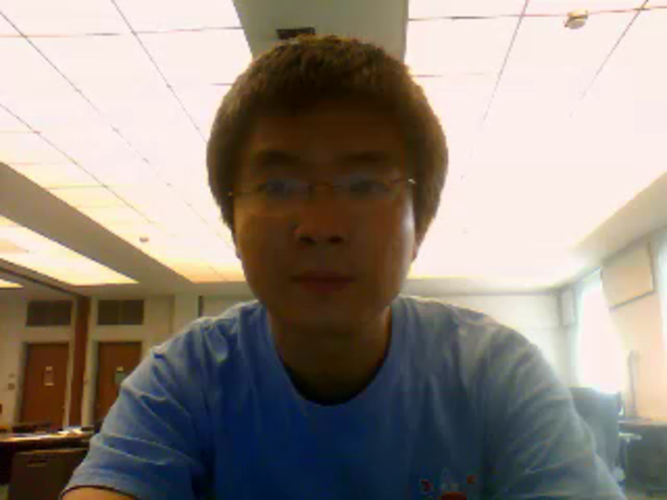
\includegraphics[scale=0.15]{ziyuan.pdf}} \\
        Ziyuan Wang\\
        
        {\centering 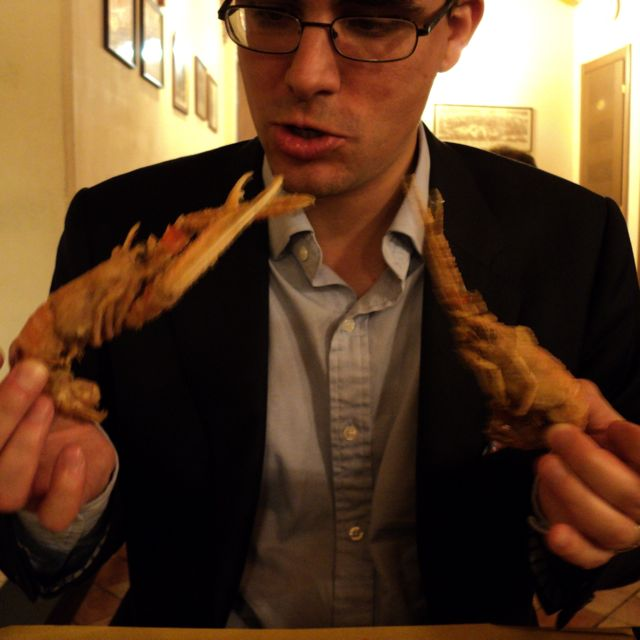
\includegraphics[scale=0.06]{adam.jpg}} \\
        Adam Lopez\\
        
        {\centering 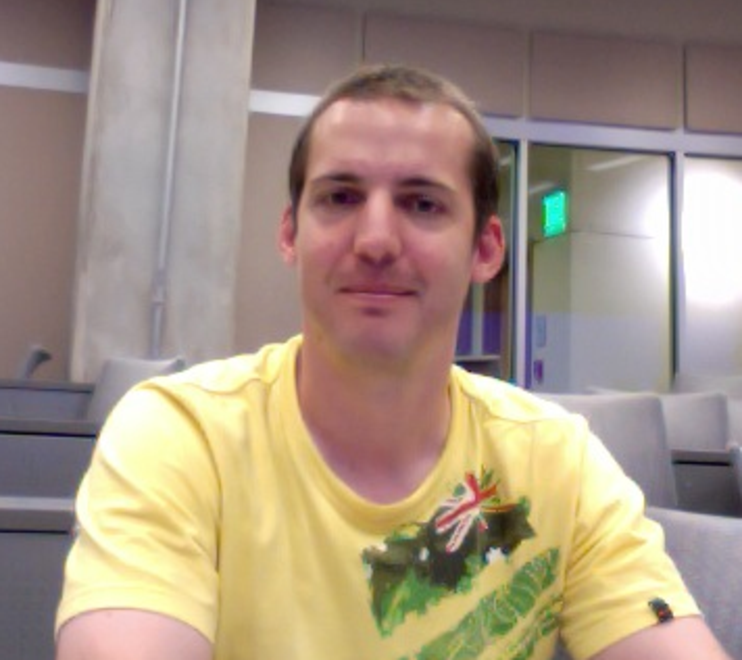
\includegraphics[scale=0.10]{jon.pdf}} \\
        Jon Graehl\\
        
        {\centering 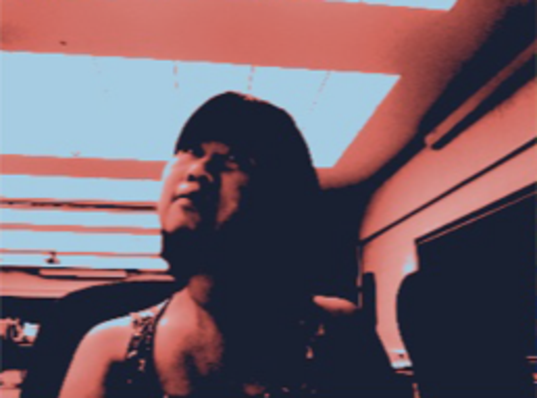
\includegraphics[scale=0.15]{linh.pdf}} \\
        ThuyLinh Nguyen\\

      \end{figure}
    \end{exampleblock}
  \vspace{0.25in}
  \end{column}
  \begin{column}{0.7\textwidth}
    \begin{itemize}
    \setlength{\itemsep}{25pt}
    \setlength{\parskip}{0pt}
    \setlength{\parsep}{0pt}
    \only<1>{\item \alert{3:15pm Training models with rich features spaces. Vlad}}
    \only<2->{\item 3:15pm Training models with rich features spaces. Vlad}
    \only<2>{\item \alert{3:30pm Decoding with complex grammars. Adam}}
    \only<1,3->{\item \alert{4:00pm Closing remarks. Phil}
    \only<3>{\item 4:05pm Finish.}
    \only<>{\item 4:05pm Finish.}
    \end{itemize}
  \end{column}
\end{columns}
\end{frame}

\begin{frame}[t]{Statistical machine translation: state-of-the-art}
%\vspace{1.0cm}
\begin{exampleblock}{Urdu $\rightarrow$ English}
  \begin{figure}
    {\centering 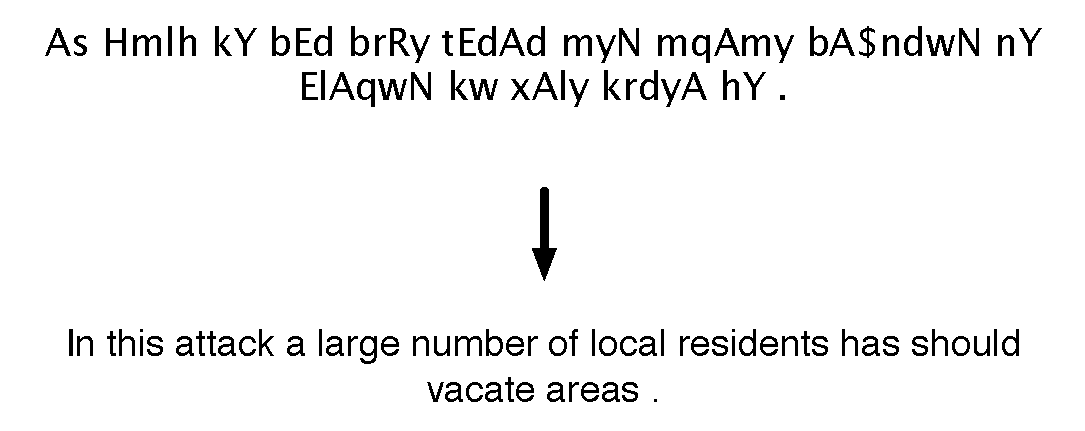
\includegraphics[scale=0.55]{urdu-bl.pdf}}
  \end{figure}
\end{exampleblock}
\begin{itemize}
  \item Current state-of-the-art translation models struggle with language pairs which exhibit large differences in structure.
\end{itemize}
\end{frame}

\begin{frame}[t]{Statistical machine translation: our unsupervised grammars}
%\vspace{1.0cm}
\begin{exampleblock}{Urdu $\rightarrow$ English}
  \begin{figure}
    {\centering 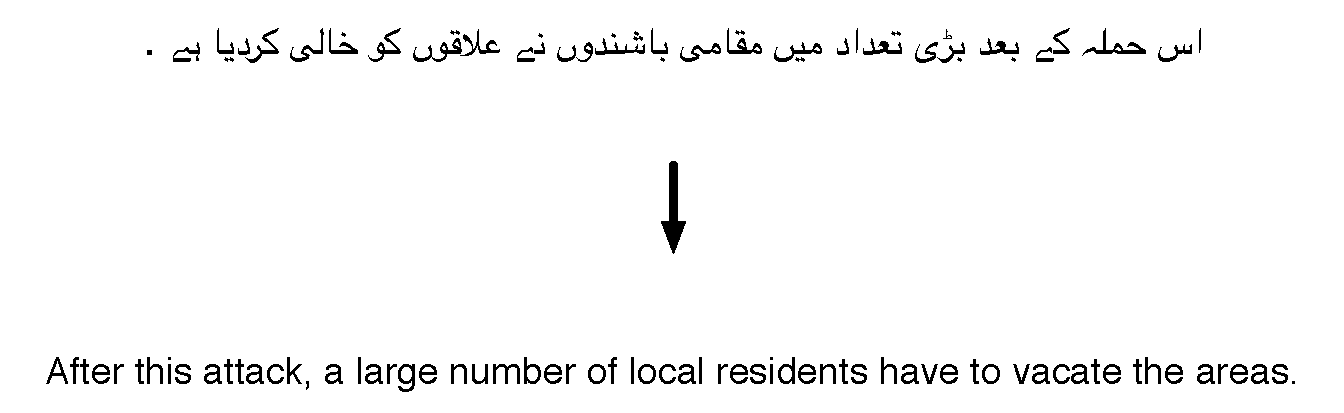
\includegraphics[scale=0.55]{urdu-25hp.pdf}}
  \end{figure}
\end{exampleblock}
\begin{itemize}
  \item In this workshop we've made some small steps towards better translations for difficult language pairs.
\end{itemize}
\only<2->{
  Google Translate: \\
  \hspace{0.25in} {\em *After the attack a number of local residents has blank areas.}
}
\end{frame}


\begin{frame}[t]{Induced Translation Structure}
\begin{center}
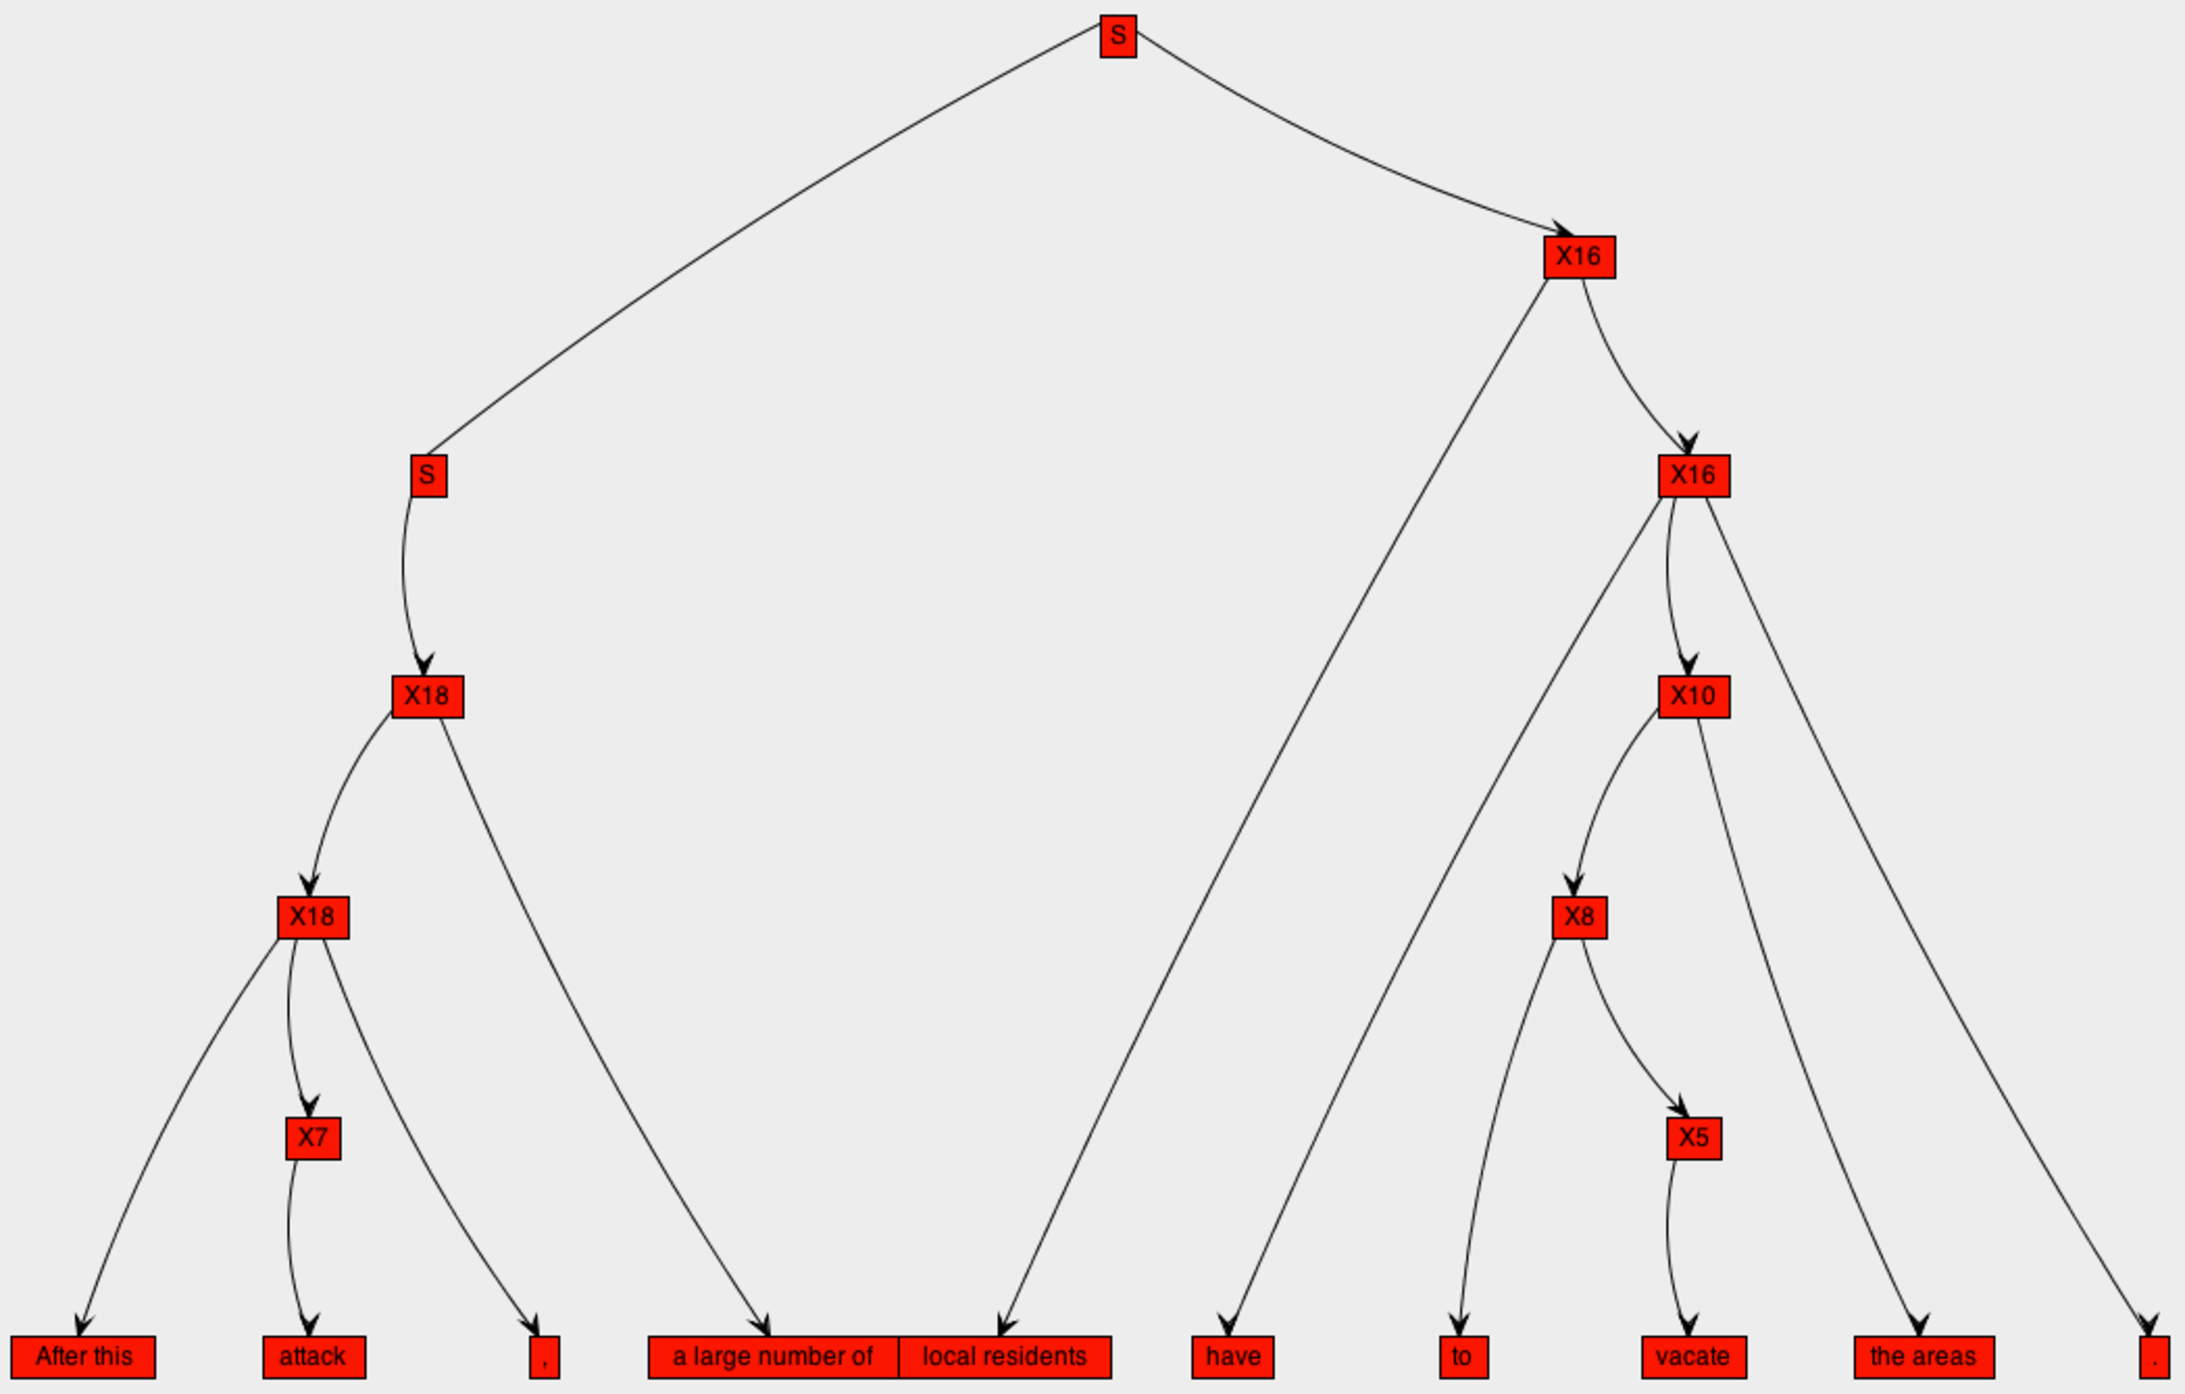
\includegraphics[scale=0.32]{joshua_tree19.pdf}
\end{center}
\end{frame}

\begin{frame}[t]{What we've achieved:}
  \vspace{0.5in}
  \begin{unpacked_itemize}
    \item 
    \item
  \end{unpacked_itemize}
\end{frame}


\begin{frame}[t]{We're we'll go from here:}
  \vspace{0.5in}
  \begin{unpacked_itemize}
    \item 
    \item 
  \end{unpacked_itemize}
\end{frame}



\end{document}
